%% This is file `elsarticle-template-1-num.tex',
%%
%% Copyright 2009 Elsevier Ltd
%%
%% This file is part of the 'Elsarticle Bundle'.
%% ---------------------------------------------
%%
%% It may be distributed under the conditions of the LaTeX Project Public
%% License, either version 1.2 of this license or (at your option) any
%% later version.  The latest version of this license is in
%%    http://www.latex-project.org/lppl.txt
%% and version 1.2 or later is part of all distributions of LaTeX
%% version 1999/12/01 or later.
%%
%% Template article for Elsevier's document class `elsarticle'
%% with numbered style bibliographic references
%%
%% $Id: elsarticle-template-1-num.tex 149 2009-10-08 05:01:15Z rishi $
%% $URL: http://lenova.river-valley.com/svn/elsbst/trunk/elsarticle-template-1-num.tex $
%%

%% Use the option review to obtain double line spacing
\documentclass[preprint]{elsarticle}
\usepackage[cm]{fullpage}

%% Use the options 1p,twocolumn; 3p; 3p,twocolumn; 5p; or 5p,twocolumn
%% for a journal layout:
%% \documentclass[final,1p,times]{elsarticle}
%% \documentclass[final,1p,times,twocolumn]{elsarticle}
%% \documentclass[final,3p,times]{elsarticle}
%% \documentclass[final,3p,times,twocolumn]{elsarticle}
%% \documentclass[final,5p,times]{elsarticle}
%% \documentclass[final,5p,times,twocolumn]{elsarticle}

%% The graphicx package provides the includegraphics command.
\usepackage{graphicx}
%% The amssymb package provides various useful mathematical symbols
\usepackage{amssymb}
%% The amsthm package provides extended theorem environments
%% \usepackage{amsthm}

%% The lineno packages adds line numbers. Start line numbering with
%% \begin{linenumbers}, end it with \end{linenumbers}. Or switch it on
%% for the whole article with \linenumbers after \end{frontmatter}.
\usepackage{lineno}

\usepackage{amsopn} % DeclareMathOperator
\usepackage{amsmath} % bmatrix

\DeclareMathOperator{\Var}{Var}
\newcommand{\effectvector}{\hat\beta}
\newcommand{\effect}[1][i]{\effectvector_{#1}}
\newcommand{\vareffect}[1][i]{\hat S^2_{#1}}
\newcommand{\zeffect}[1][\studyidx]{Z_{#1}}
\newcommand{\peffect}[1][\studyidx]{P_{#1}}
\newcommand{\nStudies}{K}
\newcommand{\studyidx}{k}
\newcommand{\varCombined}{\sigma^2_{C}}
\newcommand{\estvarCombined}{\hat\sigma^2_{C}}

\newcommand{\metaanalyticeffect}{\gamma}

\newcommand{\varBetween}{\tau^2}
\newcommand{\estvarBetween}{\hat\tau^2}
\newcommand{\varWithinCommon}{\sigma^2}
\newcommand{\sampleSize}[1][i]{n_{#1}}
\newcommand{\varWithin}[1][i]{\sigma^2_{#1}}
\newcommand{\transpose}{^T}

\newcommand{\IGE}{IGE}
\newcommand{\ISE}{ISE}

%% natbib.sty is loaded by default. However, natbib options can be
%% provided with \biboptions{...} command. Following options are
%% valid:

%%   round  -  round parentheses are used (default)
%%   square -  square brackets are used   [option]
%%   curly  -  curly braces are used      {option}
%%   angle  -  angle brackets are used    <option>
%%   semicolon  -  multiple citations separated by semi-colon
%%   colon  - same as semicolon, an earlier confusion
%%   comma  -  separated by comma
%%   numbers-  selects numerical citations
%%   super  -  numerical citations as superscripts
%%   sort   -  sorts multiple citations according to order in ref. list
%%   sort&compress   -  like sort, but also compresses numerical citations
%%   compress - compresses without sorting
%%
%% \biboptions{comma,round}

% \biboptions{}

\journal{Journal Name}

\begin{document}

\begin{frontmatter}

%% Title, authors and addresses

\title{Minimal Data Needed for Valid \& Accurate Image-Based fMRI Meta-Analysis}

%% use the tnoteref command within \title for footnotes;
%% use the tnotetext command for the associated footnote;
%% use the fnref command within \author or \address for footnotes;
%% use the fntext command for the associated footnote;
%% use the corref command within \author for corresponding author footnotes;
%% use the cortext command for the associated footnote;
%% use the ead command for the email address,
%% and the form \ead[url] for the home page:
%%
%% \title{Title\tnoteref{label1}}
%% \tnotetext[label1]{}
%% \author{Name\corref{cor1}\fnref{label2}}
%% \ead{email address}
%% \ead[url]{home page}
%% \fntext[label2]{}
%% \cortext[cor1]{}
%% \address{Address\fnref{label3}}
%% \fntext[label3]{}


%% use optional labels to link authors explicitly to addresses:
%% \author[label1,label2]{<author name>}
%% \address[label1]{<address>}
%% \address[label2]{<address>}

\author{Camille Maumet}
\author{Thomas Nichols}

\address{WMG, University of Warwick, Coventry, UK}
\address{Statistics Department, University of Warwick, Coventry, UK.}

\begin{abstract}
%% Text of abstract
Meta-analysis is a powerful statistical tool to combine results from a set of studies. When image data is available for each study, a number of approaches have been proposed to perform such meta-analysis including combination of standardised statistics, just effect estimates or both effects estimates and their sampling variance. While the latter is the preferred approach in the statistical community, often only standardised estimates are shared, reducing the possible meta-analytic approaches. Given the growing interest in data sharing in the neuroimaging community there is a need to identify what is the minimal data to be shared in order to allow for future image-based meta-analysis. In this paper, we compare the validity and the accuracy of eight meta-analytic approaches on simulated and real data. In one-sample tests, combination of contrast estimates into a random-effects General Linear Model or non-parametric statistics provide a good approximation of the reference approach. If only standardised statistical estimates are shared, permutations of z-score is the preferred approach.
\end{abstract}

\begin{keyword}
Science \sep Publication \sep Complicated
%% keywords here, in the form: keyword \sep keyword

%% MSC codes here, in the form: \MSC code \sep code
%% or \MSC[2008] code \sep code (2000 is the default)

\end{keyword}

\end{frontmatter}

%%
%% Start line numbering here if you want
%%
\linenumbers

%% main text
\section{Introduction}

TODO: check number of meta-analytic approaches (8 or 9) and update everywhere

A growing literature is focusing on the lack of statistical power in neuroimaging studies (see, e.g.~\cite{Button2013}), feeding the debate on the validity and reproducibility of published neuroimaging results. Meta-analysis, by providing inference based on the results of previously conducted studies, provides an essential method to increase power and hence confidence in neuroimaging.

A number of methods have been proposed for neuroimaging meta-analysis (see~\cite{Radua2012} for a review). As the results of neuroimaging studies are usually conveyed by providing a table of peak coordinate and statistics, most of these meta-analyses are restricted to combining coordinate-based information. Nevertheless the best practice method is an Intensity-Based Meta-Analysis (IBMA) that combines the effect estimates and their standard errors from each study~\cite{Salimi-khorshidi2009}. 

In order for IBMA to be possible in neuroimaging, tools for sharing 3D volumes obtained as a result of a statistical analysis are needed. Various efforts are currently underway to facilitate sharing of neuroimaging data but emphasis is usually on statistical maps (see, e.g. [2]). There are three evident approaches to sharing summary data from each study $i$:
\begin{enumerate}
	\item the contrast estimates $\effect$ and contrast variance estimates $\vareffect$.
	\item the contrast estimates $\effect$.	
	\item the standardized statistical maps $\zeffect$.		
\end{enumerate}

Depending on how much data is shared, different strategies can be used to combine the available results into a meta-analysis. While the first option is the best practice, leading to statistically optimal estimates~\cite{Cummings2004}, it requires the contrasts to be expressed with in the same units. In fMRI, units will depends on data, model and contrast vector scaling and are typically different across neuroimaging software due to different data scaling approaches~\cite{Nichols2012units}.


TODO: units also depend on field strength: 3T/7T
TODO: cite Gang's paper

Given the growing interest in data sharing in the neuroimaging community, and the relative easiness of sharing just (unitless) statistic maps, there is a need to identify what is the minimal data to be shared in order to allow for future IBMA.

Here we compare the use of IMBA using 9 meta-analytic approaches: 2 approaches use $\effect$'s and $\vareffect$'s, 2 $\effect$'s only and 5 $\zeffect$'s. We compare the validity and the accuracy of the eight meta-analytic approaches on simulated and real data including 21 studies of pain in control subjects.

Section~\ref{sec_meth} describes the meta-analytic estimates along with the experiments undertaken on simulated and real data to assert their validity. The results are described in section~\ref{sec_res}. Finally, we conclude in section~\ref{sec_ccl}.

\begin{figure}[t]
	\centering
% 	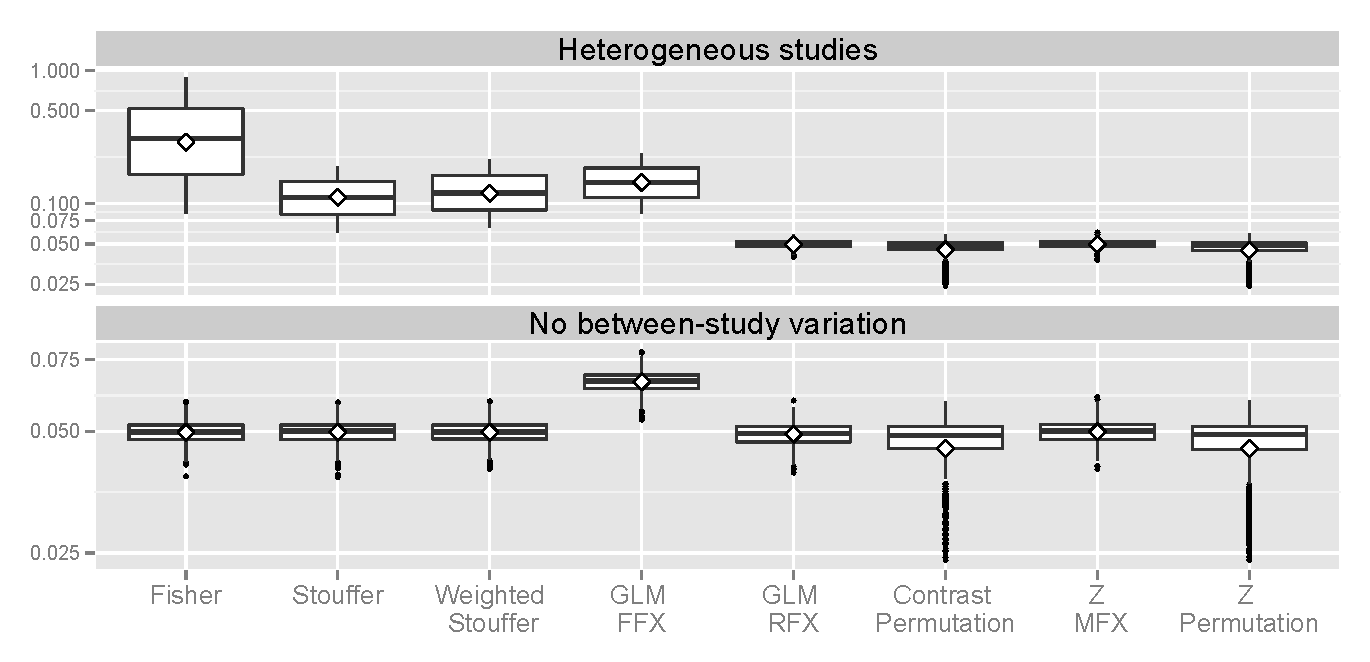
\includegraphics[width=\linewidth]{./MICCAI_version/Rplot_FPR_all.pdf}
	\caption{False positive rates of the meta-analytic estimators under the null hypothesis for $p<0.05$.}
	\label{fig_fpr_all}
\end{figure}

\section{Methods}\label{sec_meth}
\subsection{Theory}
For study $i=1,\ldots,k$ we have contrast estimate $\effect$, its contrast variance estimate $\vareffect$ (i.e. squared standard error), its statistic map $Z_i$ and its sample size $n_i$.  

\paragraph{Combining contrast estimates and their standard error}

The gold standard approach is to fit contrast estimates and their standard error with a hierarchical general linear model (GLM)~\cite{Cummings2004}, creating a third-level (level ~1:~subject; level~2:~study; level~3:~meta-analysis). The general formulation for the study-level data is:

\begin{equation}
	\vec{\effectvector} = X \metaanalyticeffect + \epsilon
	\label{eq_meta_GLM}
\end{equation}
where $\metaanalyticeffect$ is the meta-analytic parameter to estimate, $\vec{\effectvector} = [\effect[1] \ldots \effect[\nStudies] ]\transpose$ is the vector of contrast estimates, $X$ is the $k\times p$ study-level matrix (typically just a column of ones for a one-sample test) and $\epsilon \sim \mathcal{N}(0,W)$ is the residual error term. Eq.~\eqref{eq_meta_GLM} can be solved by weighted least squares giving:

TODO: add contrast

\begin{eqnarray}
	\hat \metaanalyticeffect  &=& (X\transpose W^{-1} X)^{-1} X\transpose W^{-1} \effectvector \\
	\Var(\hat \metaanalyticeffect)  &=& (X\transpose W^{-1} X)^{-1}
	\label{eq_WLS}
\end{eqnarray}

In a random-effects (RFX) meta-analysis, we have $W = \mathrm{diag}( \varWithin[1] + \varBetween, \ldots ,\varWithin[\nStudies] + \varBetween )$ where $\varBetween$ denotes the between-study variance. Approximating $\varWithin$ by $\vareffect$ and given $\estvarBetween$ an estimate of $\varBetween$ we obtain the statistics detailed in Table~\ref{stat_table} for one-sample tests. This reference approach will be referred to as \textbf{Mixed-effects (MFX) GLM}.
In a \textbf{fixed-effects (FFX) GLM} (i.e. assuming no or negligible between-study variance), we have $W = \mathrm{diag}( \varWithin[1] \ldots \varWithin[\nStudies] )$ where $\varWithin$ denotes the contrast variance for study $i$. 

TODO: need to state the assumptions (e.g. within-study is the true within study var?)

TODO: We need a second table for two-sample tests

\begin{table*}[t]
\begin{center}
\setlength{\tabcolsep}{3pt}
\begin{tabular}{ccccl}
				& Meta-analysis statistic			& Nominal H$_0$ distrib. & Inputs & Assumptions\\
\hline						
FFX GLM 		& $  \left(  \sum_{i=1}^\nStudies  \frac{\effect}{\vareffect} \right) / \sqrt{\sum_{i=1}^\nStudies 1/\vareffect } $ & $\mathcal{T}_{ (\sum_{i=1}^\nStudies n_i - 1) - 1}$ & $\effect, \vareffect$ 
& IGE; $\varWithin$ cst; $\varBetween=0$.\\
MFX GLM 		& $ \left( \sum_{i=1}^\nStudies \frac{\effect}{\vareffect + \estvarBetween} \right)/ \sqrt{\sum_{i=1}^\nStudies 1/ (\vareffect + \estvarBetween) } $ & $\mathcal{T}_{\nStudies - 1}$ & $\effect, \vareffect$& IGE; $\varBetween=\estvarBetween$.\\
RFX GLM 		& $  \left( \sum_{i=1}^\nStudies \frac{\effect}{\sqrt{\nStudies} } \right) / \widehat\varCombined  $ & $\mathcal{T}_{\nStudies - 1}$ & $\effect$ & IGE; $\varBetween+\varWithin$ cst.\\
Ctrst Perm.	& $ \left( \sum_{i=1}^\nStudies \frac{\effect}{\sqrt{\nStudies}} \right) /\widehat\varCombined  $ & Empirical & $\effect$ & ISE.\\
Fisher's	& $ \displaystyle -2 \sum_{\studyidx} \ln \peffect $ & $\chi^2_{(2\nStudies)}$ & $\zeffect$ & IGE; $\varBetween=0$.\\
Stouffer's& $ \displaystyle \sqrt{\nStudies} \times \frac{1}{\nStudies} \sum_{\studyidx} \zeffect $ & $\mathcal{N}(0,1)$ & $\zeffect$& IGE; $\varBetween=0$.\\
Wght Stouff.& $  \displaystyle \frac{1}{\sqrt{\sum_{\studyidx} n_\studyidx}} \sum_{\studyidx}  \sqrt{n_\studyidx} \zeffect  $ & $\mathcal{N}(0,1)$ & $\zeffect, \sampleSize$& IGE; $\varBetween=0$.\\
Z MFX& $ \left(   \sum_{i=1}^\nStudies \zeffect \right)/ \sqrt{\nStudies} \hat \sigma$ & $\mathcal{T}_{\nStudies-1}$ & $\zeffect$& IGE; $1 + \varBetween/\varWithin$ cst.\\
Z Perm.	& $\left(  \sum_{i=1}^\nStudies \zeffect \right) / \sqrt{\nStudies}$ & Empirical & $\zeffect$ & ISE.\\
\hline 

\end{tabular}
\end{center}
\caption{Statistics for one-sample meta-analysis tests and their sampling distributions under the null hypothesis $H_0$. Empirical null distributions are determined using permutations with sign flipping. \IGE=Independent Gaussian Errors, \ISE=Independent Symmetric Errors. Note: $\peffect = \Phi(-\zeffect)$}
\label{stat_table}
\end{table*}	

\paragraph{Combining contrast estimates}
If the $\vareffect$ are unavailable, the contrast estimates $\effect$ can be combined by assuming that the within-study contrast variance $\varWithin$ is roughly constant ($\varWithin \simeq \sigma^2$) or negligible in comparison to the between-study variance($\varWithin \ll \varBetween$). Then $W = \mathrm{diag}( \varCombined, \ldots, \varCombined )$ where $\varCombined$ is the combined within and between-subject variance, i.e.\ $\varCombined \simeq \varBetween$ or $\varCombined \simeq \varBetween + \varWithinCommon$ (note, however, in this setting we do not separately estimate $\varBetween$ or $\varWithinCommon$). Under these assumptions, Eq.~\eqref{eq_meta_GLM} can be solved by ordinary least squares giving:

\begin{eqnarray}
	\hat \metaanalyticeffect  &=& (X\transpose X)^{-1} X\transpose \effectvector \\
	\Var(\hat \metaanalyticeffect)  &=& (X\transpose X)^{-1} \varCombined
	\label{eq_OLS}
\end{eqnarray}

Given $\estvarCombined$ an estimate of $\varCombined$ we obtain the statistics presented in Table~\ref{stat_table} for one sample tests. This approach will be referred to \textbf{RFX GLM} in the following.

As an alternative to parametric approaches, non-parametric inference~\cite{Holmes1996,Nichols2002} can be performed by comparing the RFX GLM T-statistic to the distribution obtained with ``sign flipping'', i.e.\ randomly multiplying each study's data by 1 or -1, justified by an assumption of independent studies and symmetrically distributed random error. This approach will be referred to as \textbf{Contrast permutation}.

TODO: We should be able to do something if we have the sample sizes by assuming constant within subject variance

TODO: We should be able to do something if we have the sample sizes by assuming constant within subject variance

\paragraph{Combining standardised statistics} 
When only test statistic images are available there are a several alternate approaches available. \textbf{Fisher's} meta-analysis provide a statistic to combine the associated p-values~\cite{Fisher1932}. \textbf{Stouffer's} approach combines directly the standardised statistic~\cite{Stouffer1949}. In \cite{Zaykin2011} following \cite{Liptak1958}, the author proposed a weighted method that weights each study's $\zeffect$ by the square root of its sample size [3,7]. This approach will be referred to as \textbf{Weighted Stouffer's}. All these meta-analytic statistics assumes no or negligible between-study variance and are suited only for one-sample tests. The corresponding statistics are presented in Table~\ref{stat_table}.
As suggested in~\cite{Salimi-khorshidi2009}, to get a kind of MFX with Stouffer's approach, the standardised statistical estimates $\zeffect$ can be combined in an OLS analysis. The corresponding estimate, referred as \textbf{Z MFX} is also provided in~\ref{stat_table}

With contrasts, non-parametric inference~\cite{Holmes1996,Nichols2002} can be obtained by sign flipping on the $\zeffect$'s. This approach will be referred to as \textbf{Z permutation}.

\paragraph{Approximations}  In practice, all of the methods based on contrast data have approximate parametric null distributions.  The nominal distributions listed in~Table~\ref{stat_table} are under the (unrealistic) assumption of homogeneous standard errors over studies; even if all studies are `clean' and conducted at the same center, variation in sample size will induce differences in $\vareffect$'s.  Further, even under homoscedasticity, MFX GLM's null is approximate due to iterative estimation of~$\estvarBetween$.


TODO: Clarify what is approximate in each + units issue + RFX/FFX choice

% \begin{figure}[t]
% 	\centering
% 	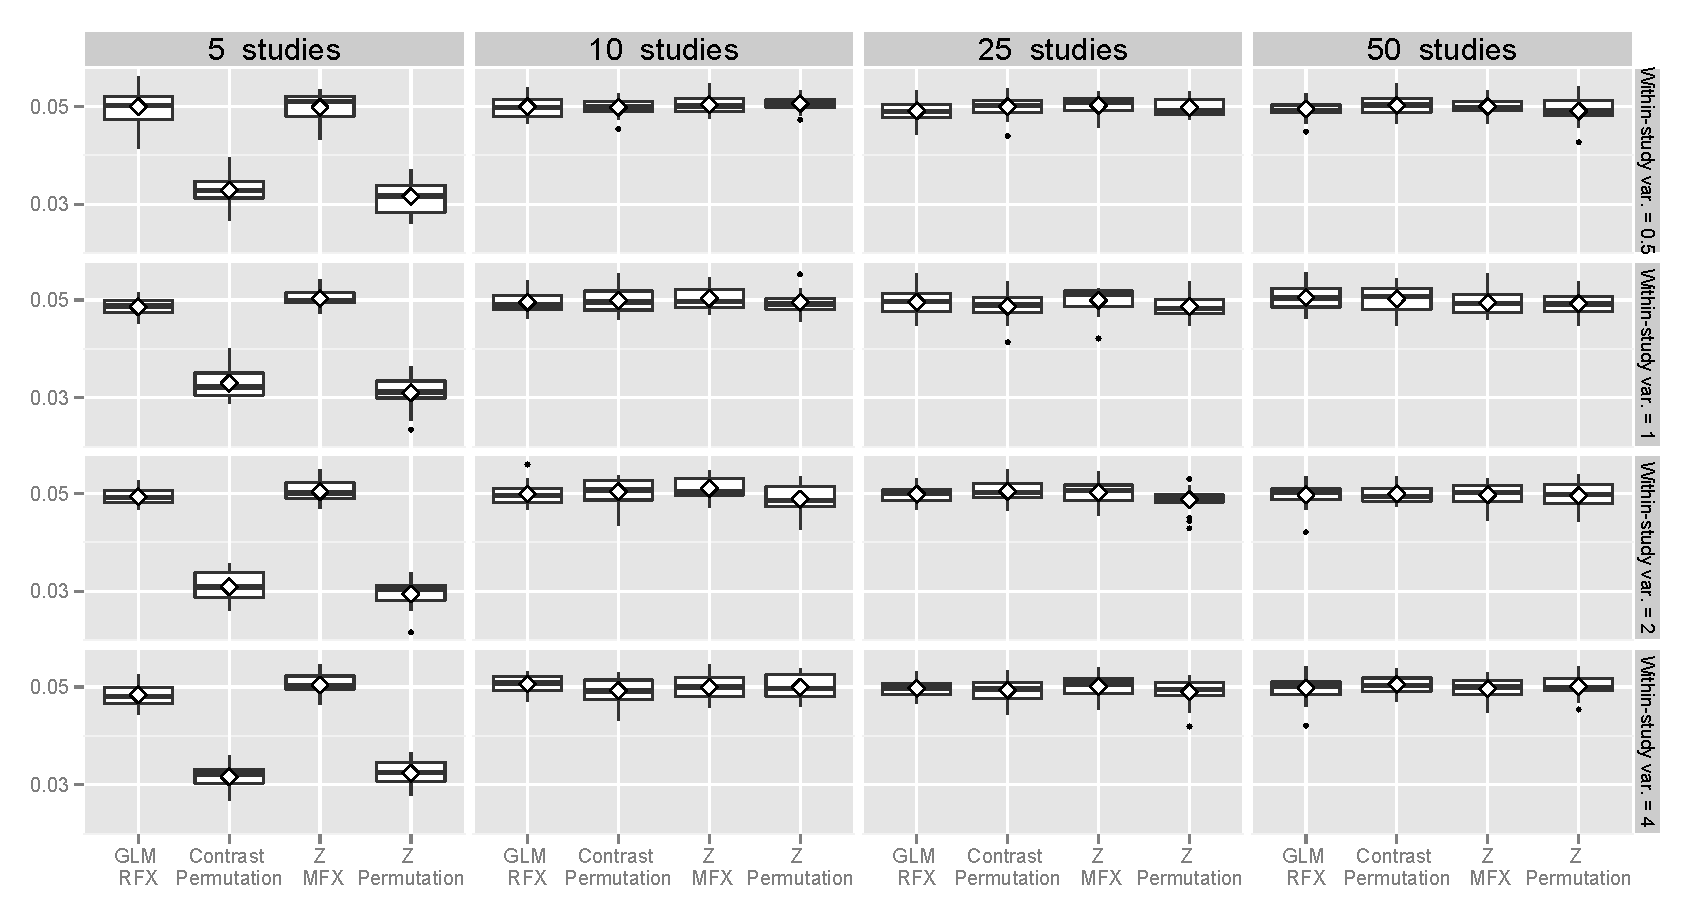
\includegraphics[width=\linewidth]{./MICCAI_version/Rplot_valids.pdf}
% 	\caption{False positive rates of the RFX meta-analytic estimators under $H_0$ for $p<0.05$ as a function of the number of studies and the within-study variance.}
% 	\label{fig_fpr_valid}
% \end{figure}

\subsection{Experiments}

\subsubsection{Simulations}
Due to the approximate nature of the sampling distributions, we conduct simulations to evaluate the validity of each estimator under inhomogeneity of contrast variances $\vareffect$ and under the presence of non-negligible between-study variance.


TODO: No longer at $p<0.05$

To verify the validity of each estimator under the null hypothesis we estimated the false positive rate at $p<0.05$ uncorrected. For each meta-analysis, we simulated $\effect$ and $\vareffect$ such as:
\begin{eqnarray}
	\effect &\sim& \mathcal{N}(0, \frac{\varWithin}{\sampleSize}+\varBetween) \\
	\vareffect &\sim& \frac{\varWithin}{\sampleSize-1} \chi^2_{(\sampleSize-1)}%
\end{eqnarray}
where $\varWithin \in [1/2, 1, 2, 4]$ is the within-study variance, $\varBetween \in [0, 1/20]$ is the between-study variance (fixed-effects models are strictly only appropriate for $\varBetween=0$). For different number of studies per meta-analysis we used: $\nStudies \in [5, 10, 25, 50]$, and set the number of subjects per studies $\sampleSize$ to vary across the common range of sample sizes in neuroimaging studies. In each simulated meta-analysis we simulated one study with exactly 20, 25, 10 and 50 subjects. For the remaining studies $1/4$ of the $\sampleSize$'s were drawn from $\mathcal{U}(11,20)$, $1/4$ from $\mathcal{U}(26,50)$ and the remaining from $\mathcal{U}(21,25)$, where $\mathcal{U}(a,b)$ is the discrete uniform distribution on the integers $a$ to $b$ inclusive. A total of 32 parameter sets (4 $\varWithin$ x 2 $\varBetween$ x 4 $\nStudies$) was therefore tested and a total of $71^3$ realisations were created.


\subsubsection{Real data}
We then compared the 8 meta-analytic estimators to the reference approach, MFX GLM, on a dataset of 21 studies of pain. 
Comparability of contrast estimates depends on equivalent scaling of the data, models, and contrast vectors. Data scaling was consistently performed by FSL, setting median brain intensity to 10,000; model were all created by FSL's Feat tool; and contrasts were constructed to preserve units, with sum of positive elements equal to 1, sum of negative elements equal to -1. 


% TODO: Anyone who knows the slightest bit about meta-analysis will know about Cochran's Q test and the I^2 test.  I think you've created some version of I^2 (maybe).  ANYWAY, it's good to mention these somewhere (intro) and say that that we propose an intuitive exploratory metric to assess heterogentiy that complents existing methods (Cochran's Q, I^2).

% See this ref: 

% Higgins, J. P. T., & Thompson, S. G. (2002). Quantifying heterogeneity in a meta-analysis. Statistics in Medicine, 21(11), 1539–58. doi:10.1002/sim.1186


To investigate the presence of between-study variation, we computed the ratio of the between-study variance (estimated using FSL's FLAME~\cite{Smith2001}) to the total variance (sum of between- and within-study variances), as suggested in~\cite{Chen2012}. Here we use the average (across study) within-study variance as an estimate of within-study variance in the denominator:
$\estvarBetween / (\estvarBetween + \sum_{i=1}^{\nStudies} \vareffect)$.
Using this metric, voxels with values close to 0 present negligible between-study variance and values close to 1 outline appreciable study heterogeneity and the importance of RFX~models.

Then for each estimator we compared the standardised meta-analytic statistic to the z-statistic obtained with the reference approach. Overestimation of z-statistic leads to overly optimistic detections while underestimation outline a reduced sensitivity of the approach. 

\begin{figure}[t]
	\centering
% 	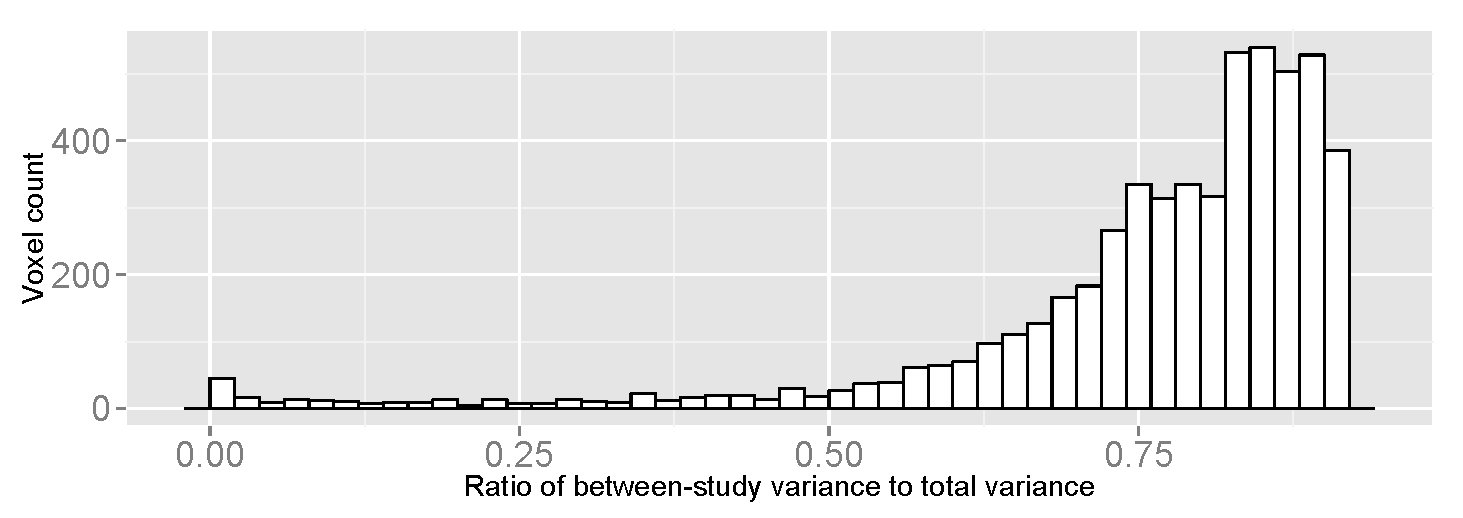
\includegraphics[width=0.7\linewidth]{./MICCAI_version/Rplot_ratio_variances.pdf}
	\caption{Histogram of the between-study variance to the sum of the between-subject variance and the mean within-study variance.}
	\label{fig_realdata_variances}
\end{figure}

\section{Results}\label{sec_res}

\subsection{How bad is the units issue?}

\subsubsection{Group meta-analysis}

\begin{figure}[t]
	\centering
	\hspace*{-1.5in}
 	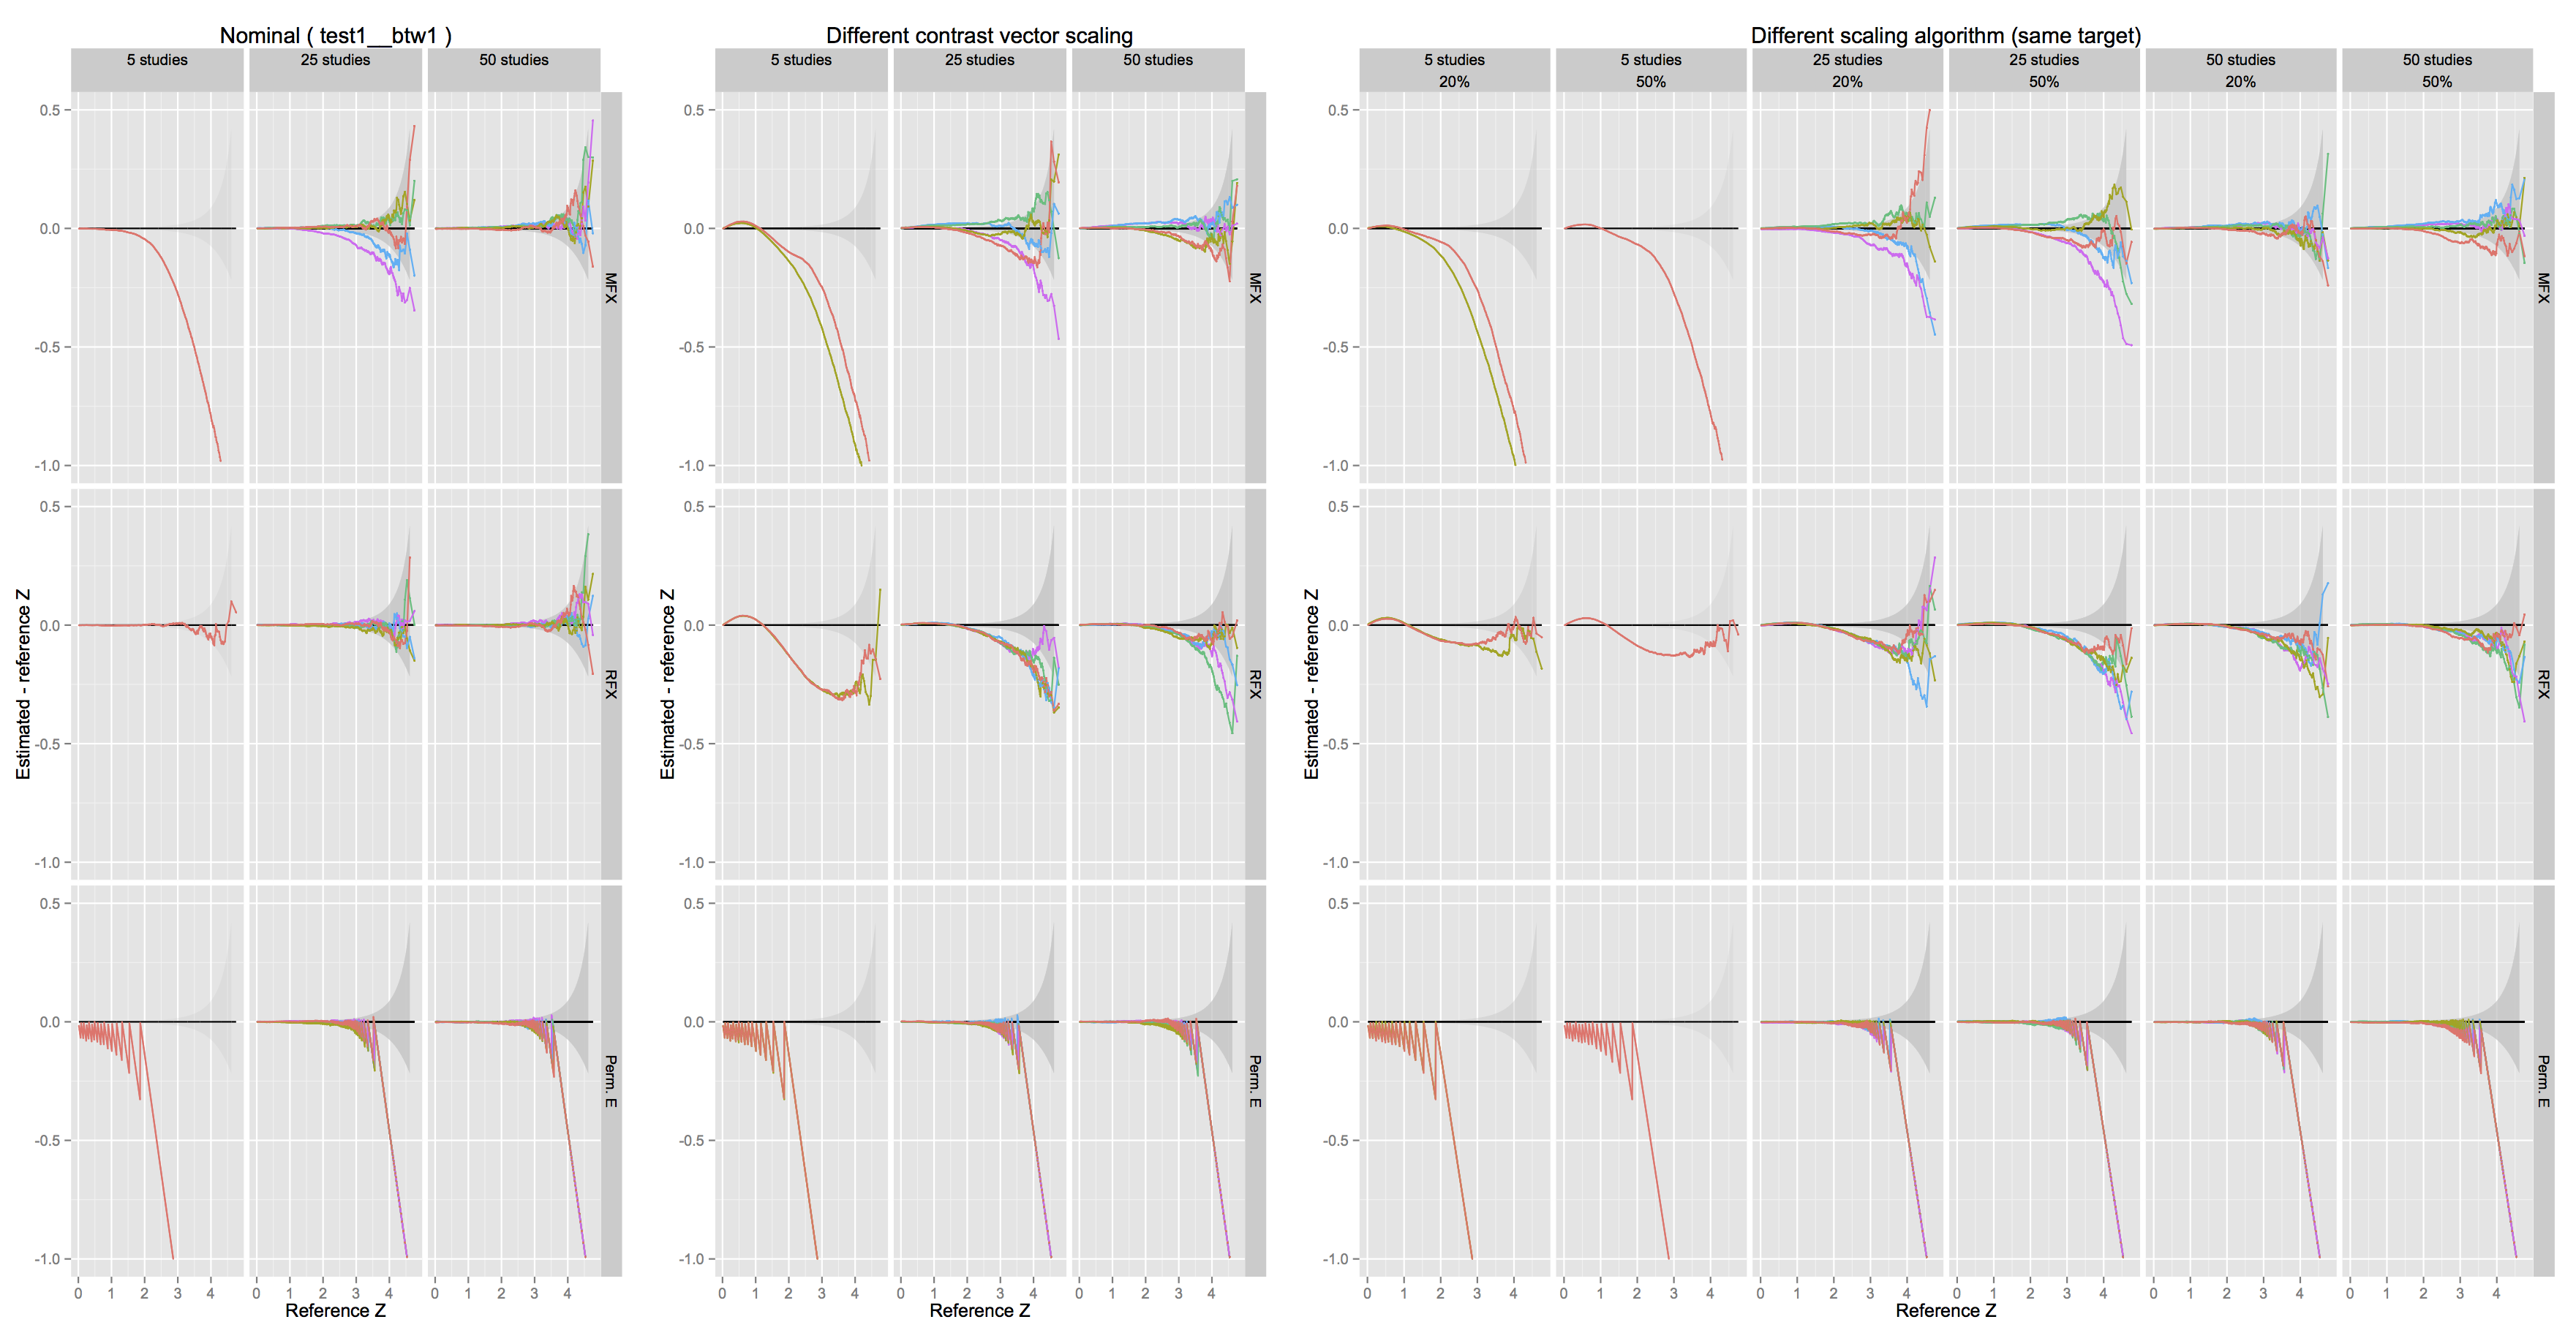
\includegraphics[width=1.3\linewidth]{./figures/test1_btw1.png}
	\caption{Deviation from theoretical Z in one-sample tests with $\varBetween=1$ and $\nStudies = 5, 25, 50$ with matched (``nominal'') or mismatched (``different scaling target", ``different scaling algorithm", ``different contrast vector scaling") units.}
	\label{test1_k25_btw1}
\end{figure}

Fig.~\ref{test1_k25_btw1} presents the simulation results for a one-sample with $\varBetween=1$ and a sample size $\nStudies = 5, 25, 50$. For the nominal case, i.e. when the units are matched across studies and contrasts, MFX GLM, RFX GLM and Contrast Permutation are all valid, as expected. For small sample sizes ($\nStudies = 5$), MFX GLM and contrast permutation are both very conservative. For large values of Z, Contrast Estimation is conservative as expected due to the discrete nature of its distribution. More suprinsing, in the presence of a high within-subject variance, MFX GLM also appears to be conservative. RFX GLM displays the best behaviour with a pattern that is always within the 95\% confidence interval of the theoretical Z.

% In the extreme case of different scaling target, i.e. when data where scaled to a different mean (100 versus 10 000), Contrast Permutation displays a pattern that is very close to its nominal behaviour, namely it is valid but conservative for large Z. GLM RFX is valid for Z values that are greater than 1.5 (i.e. the area we are interested in in terms of detections) but very conservative, especially when the number of samples from each scaling factor are not equal. This behaviour is expected as the estimated between-study variance is inflated by the difference in scaling target. MFX GLM is invalid for small within-subject variances and conservative for large within-subject variances.

When different scaling algorithm are used, i.e. with different neuroimaging software packages, Contrast Permutation still has a behaviour that is very similar to nominal. MFX GLM and RFX GLM display invalidity for small Z's and conservativness for large Z's (but less conservative than Contrast Permutation). 

When the contrast are scaled differently, we observe a very similar pattern than for different scaling algorithm.

\subsubsection{Balanced between-group meta-analysis}

Fig.~TODO presents the simulation results for a two-sample meta-analyses with $\varBetween=1$ and a sample size $\nStudies = 25$. For the nominal case, GLM RFX, GLM RFX and contrast estimation provide valid estimates. Contrast Permutation is conservative for large Z values. Both RFX GLM and MFX GLM display the best behaviour with a pattern that is within the 95\% confidence interval of the theoretical Z.

In the extreme case of different scaling target, contrast permutation is always valid with a pattern very similar than its nominal behaviour. GLM RFX is valid for Z values greater than 1.5, which is the area of interest in detections, but display a strong conservativness, more pronounced than the Contarst Permutation. GLM MFX is slighlty invalid for all within-subject variances except the largest one when 20\% of the studies come from the second software.

\begin{figure}[t]
	\centering
 	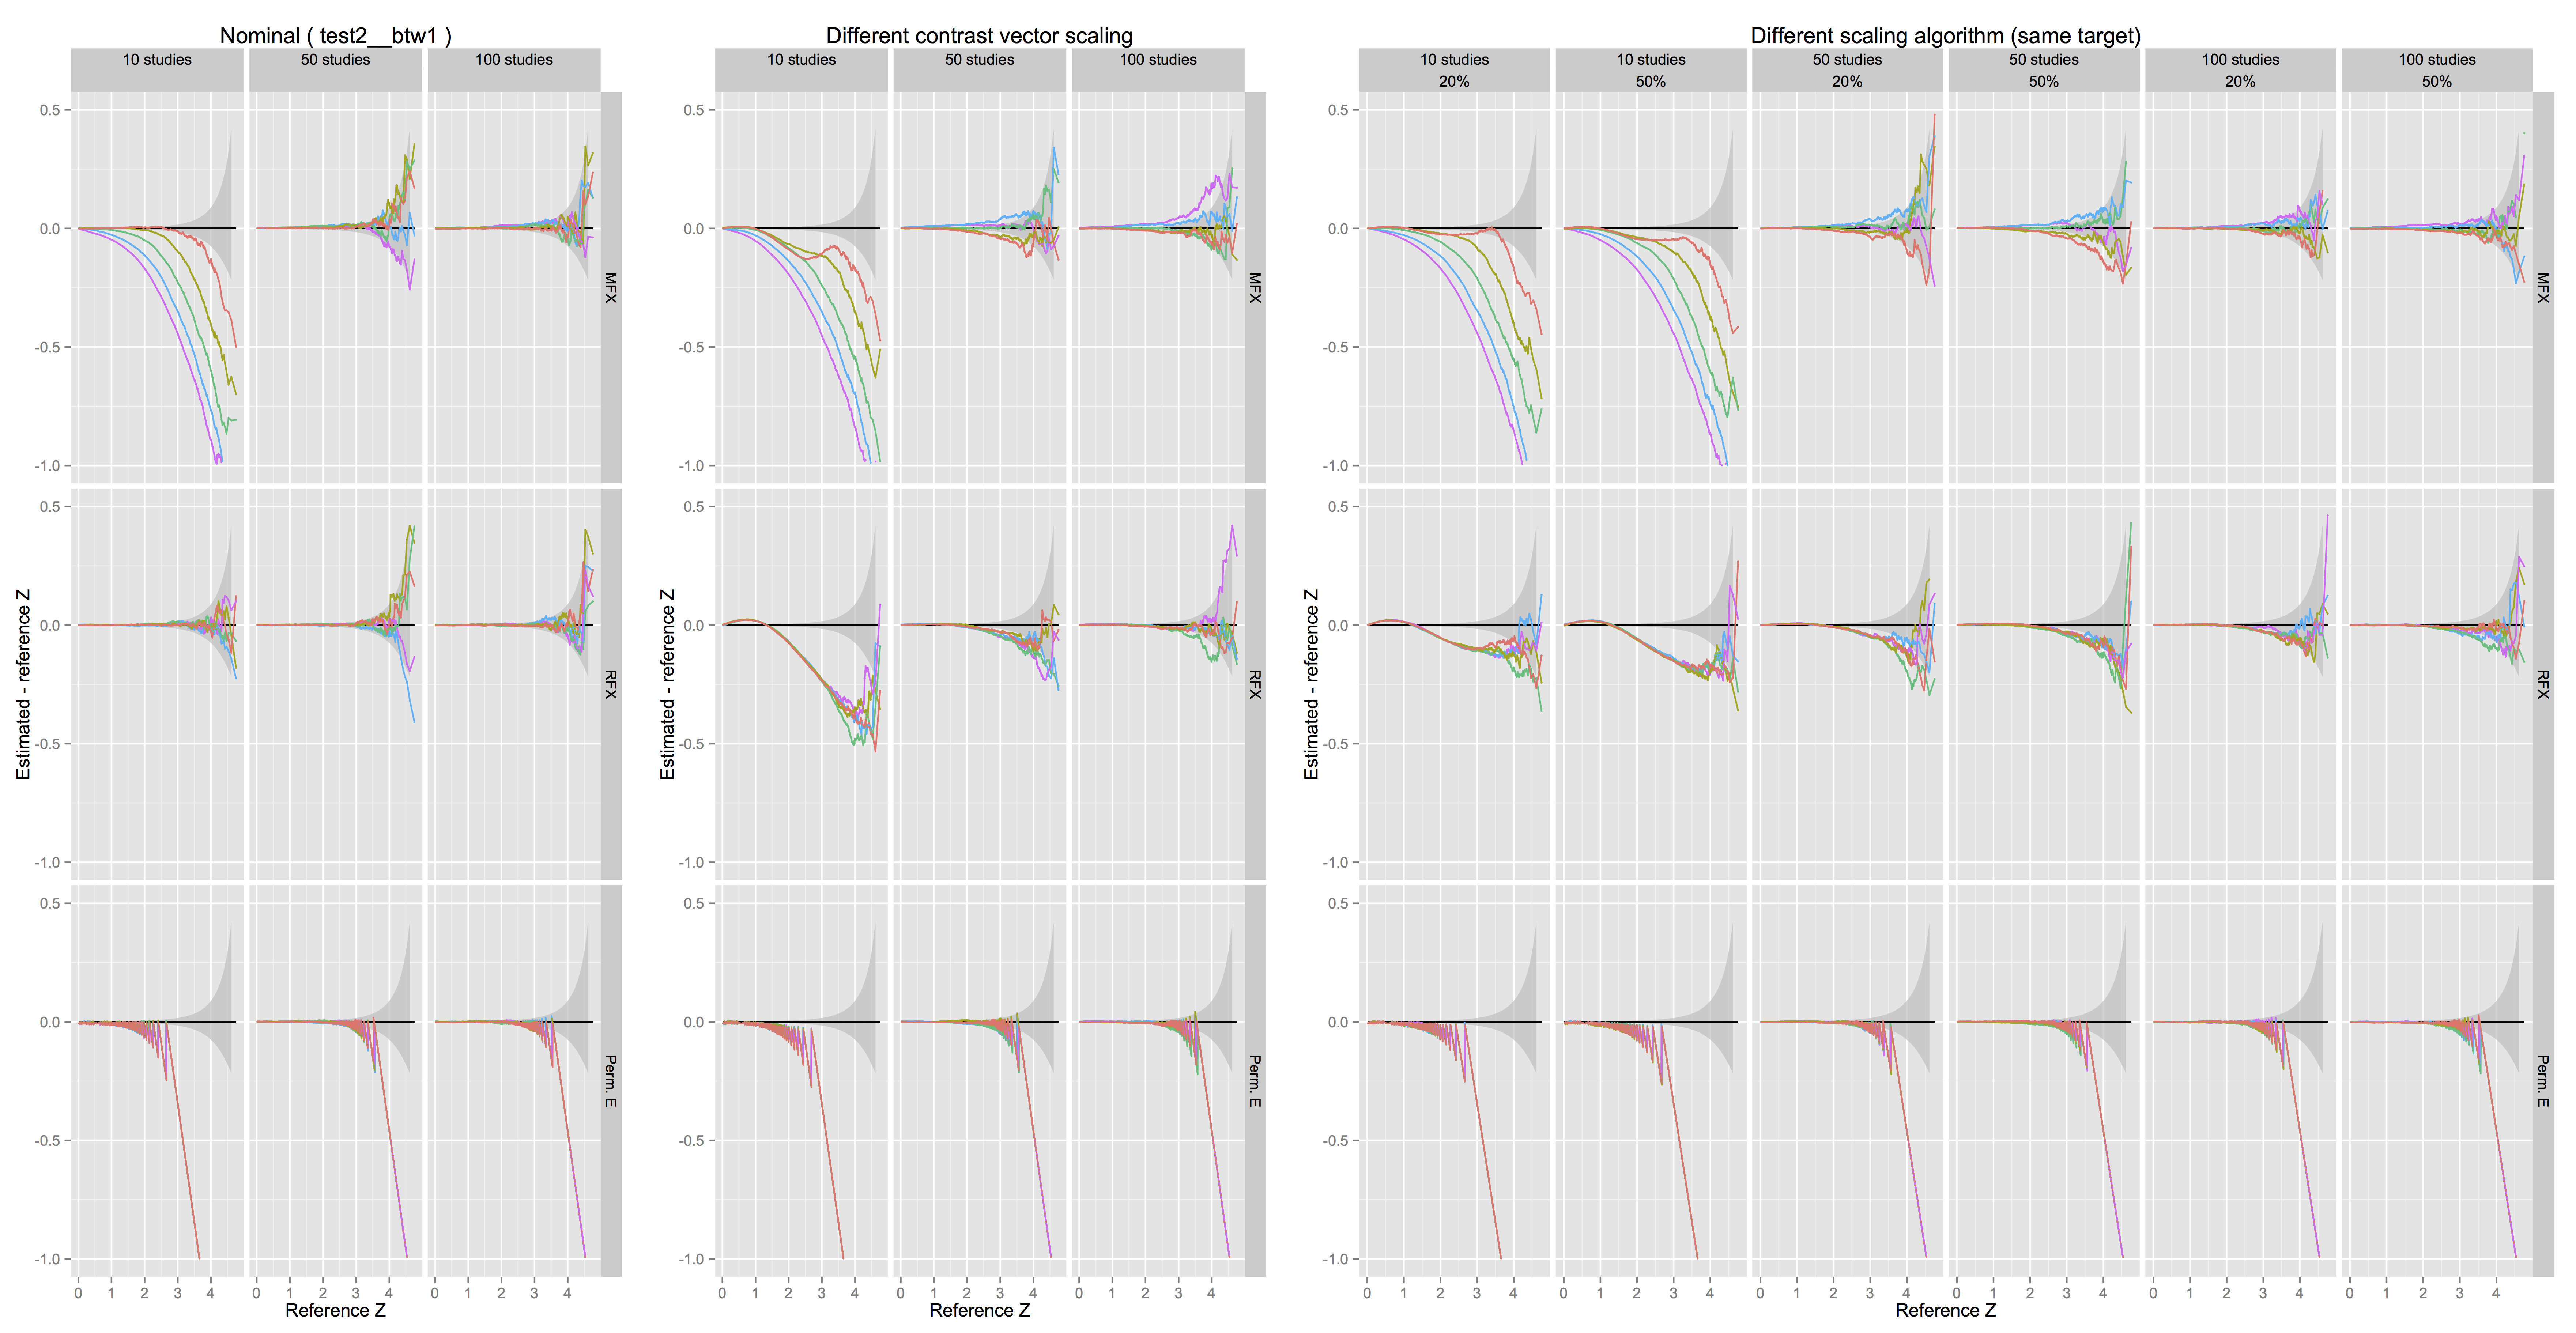
\includegraphics[width=0.99\linewidth]{./figures/test2_btw1.png}
	\caption{Deviation from theoretical Z in balanced two-sample tests with $\varBetween=1$ and $\nStudies = 25$ with matched (``nominal'') or mismatched (``different scaling target", ``different scaling algorithm", ``different contrast vector scaling") units.}
	\label{test2_btw1}
\end{figure}

\subsubsection{Unbalanced between-group meta-analysis}

\begin{figure}[t]
	\centering
 	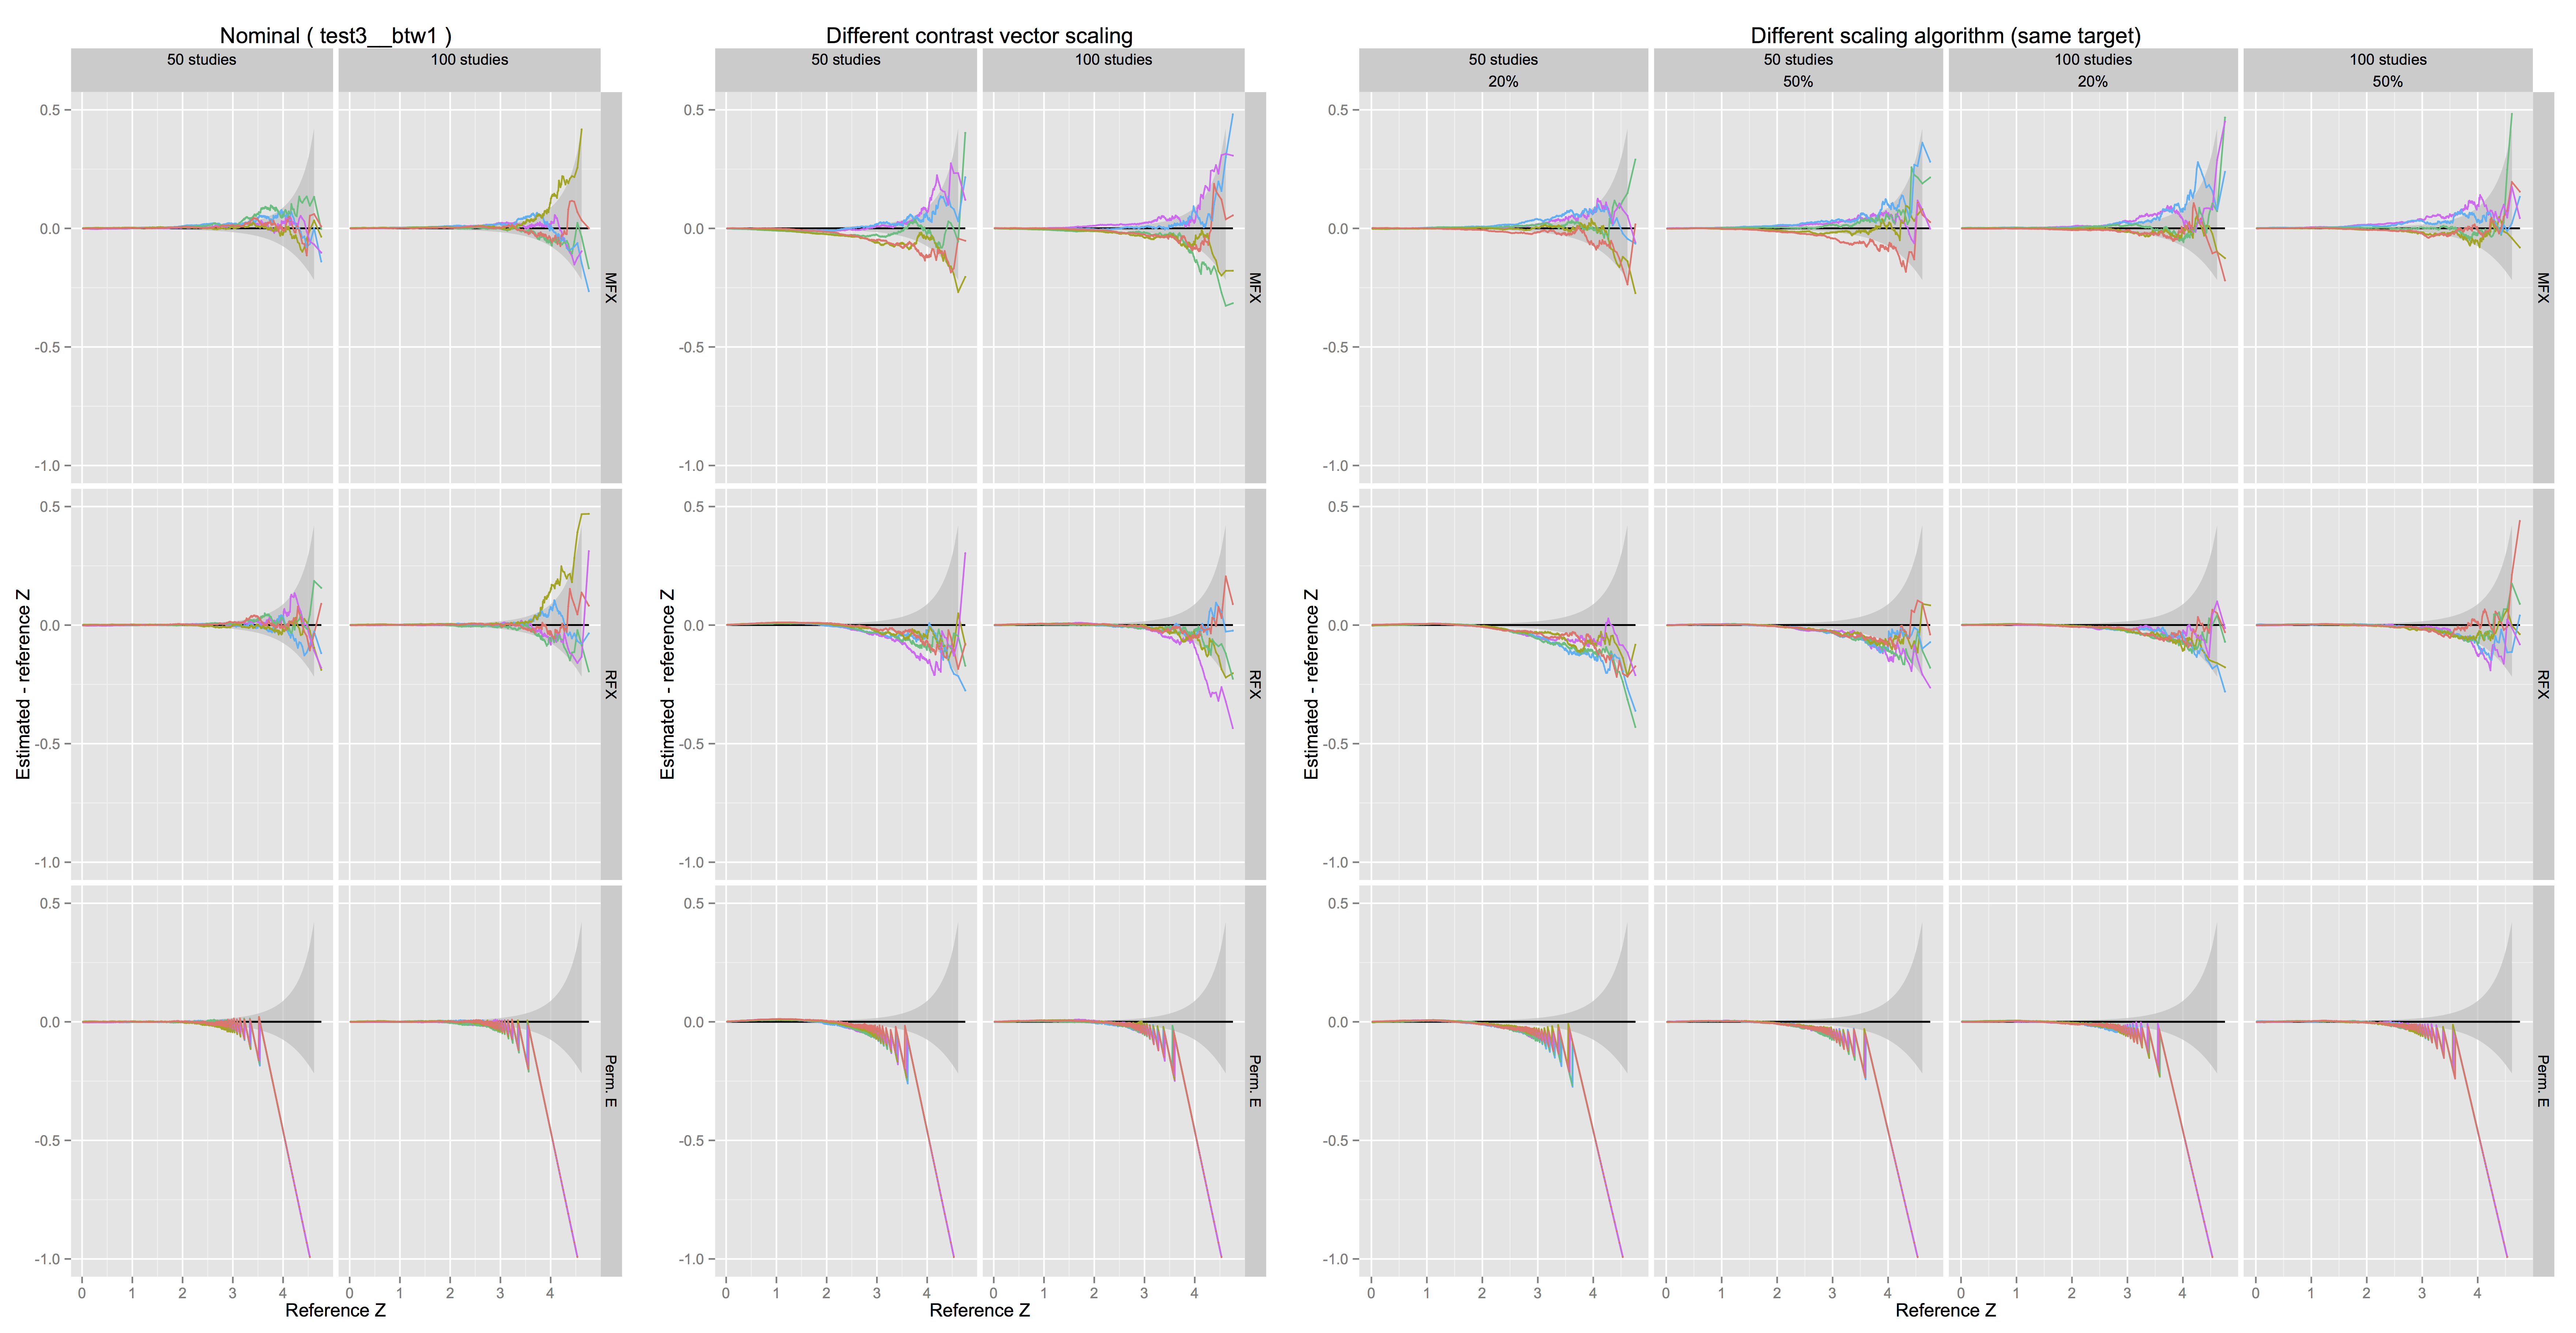
\includegraphics[width=0.99\linewidth]{./figures/test3_btw1.png}
	\caption{Deviation from theoretical Z in unbalanced two-sample tests with $\varBetween=1$ and $\nStudies = 25$ with matched (``nominal'') or mismatched (``different scaling target", ``different scaling algorithm", ``different contrast vector scaling") units.}
	\label{test3_btw1}
\end{figure}

Fig.~TODO presents the simulation results for unbalanced two-sample meta-analyses with $\varBetween=1$ and a sample size $\nStudies = 25$. For the nominal case, MFX GLM, GLM RFX and contrast permutation provide valide estimate. As expected due to the discrete nature of its ampling distribution, contrast permutation is conservative for large Z value. GLM RFX is conservative. RFX GLM is closest to the theoretical behaviour with Z-values that are always within the 95\% confidence interval.

In the extreme case of different scaling target, MFX GLM is always valid but slightly conservative. RFX GLM is valid for Z values greater than 1.5 (area of interest in detections) but conservative. Similarly contrast permutation is invalid for Z smaller than 1.5 and conservative otherwise. This can be explained by the violation of the exchangeability condition.

When different scaling algorithm are used, (same paragraph as for one-sample test)

When the contrast are scaled differently, we observe a very similar pattern than for different scaling algorithm with higher varaince of the estimates.


\subsection{Simulations}
Fig.~\ref{fig_fpr_all} displays the false positive rate at $p<0.05$ obtained for the eight estimators over all set of parameters in the absence and presence of between-study variation. As expected, the fixed-effects meta-analytic summary statistics, i.e.\ Fisher's, Stouffer's and weighted Stouffer's estimates, are liberal in the presence of study heterogeneity. The original Fisher's approach is the most invalid. More surprising, FFX GLM is also invalid with homogeneous studies. The explanation is over-estimation of degrees-of-freedom (DF); while DF is computed as $(\sum n-1)-1$, under heteroscasdicity (from $\sigma_i$ or $\sampleSize$) it will be much lower~\cite{Satterthwaite}. Z MFX and GLM RFX provide valid estimates, and the permutation estimates are valid but tend to be conservative with greater variation in false positive rates.

The impact of the number of studies involved in the meta-analysis and of the size of the within-study variance are investigated in Fig.~TODO. Permutation inference is valid but conservative when 5 studies are used; this is because there are only $2^5=32$ possible permutations and thus $1/32=0.03125$ is largest attainable valid P-value. All approaches perform equally as soon as 10 or more studies are included in the meta-analysis. 


\subsection{Real data}



The histogram of the ratio of between-subject variance to total variance is displayed in Fig.~\ref{fig_realdata_variances}. From this graph it is clear that for most of the voxels the estimated between-study variance is greater than the within-study variance. We can therefore suppose the presence of study heterogeneity (non negligible between-study variance) in this collection of studies.

\begin{figure}[t]
	\centering
% 	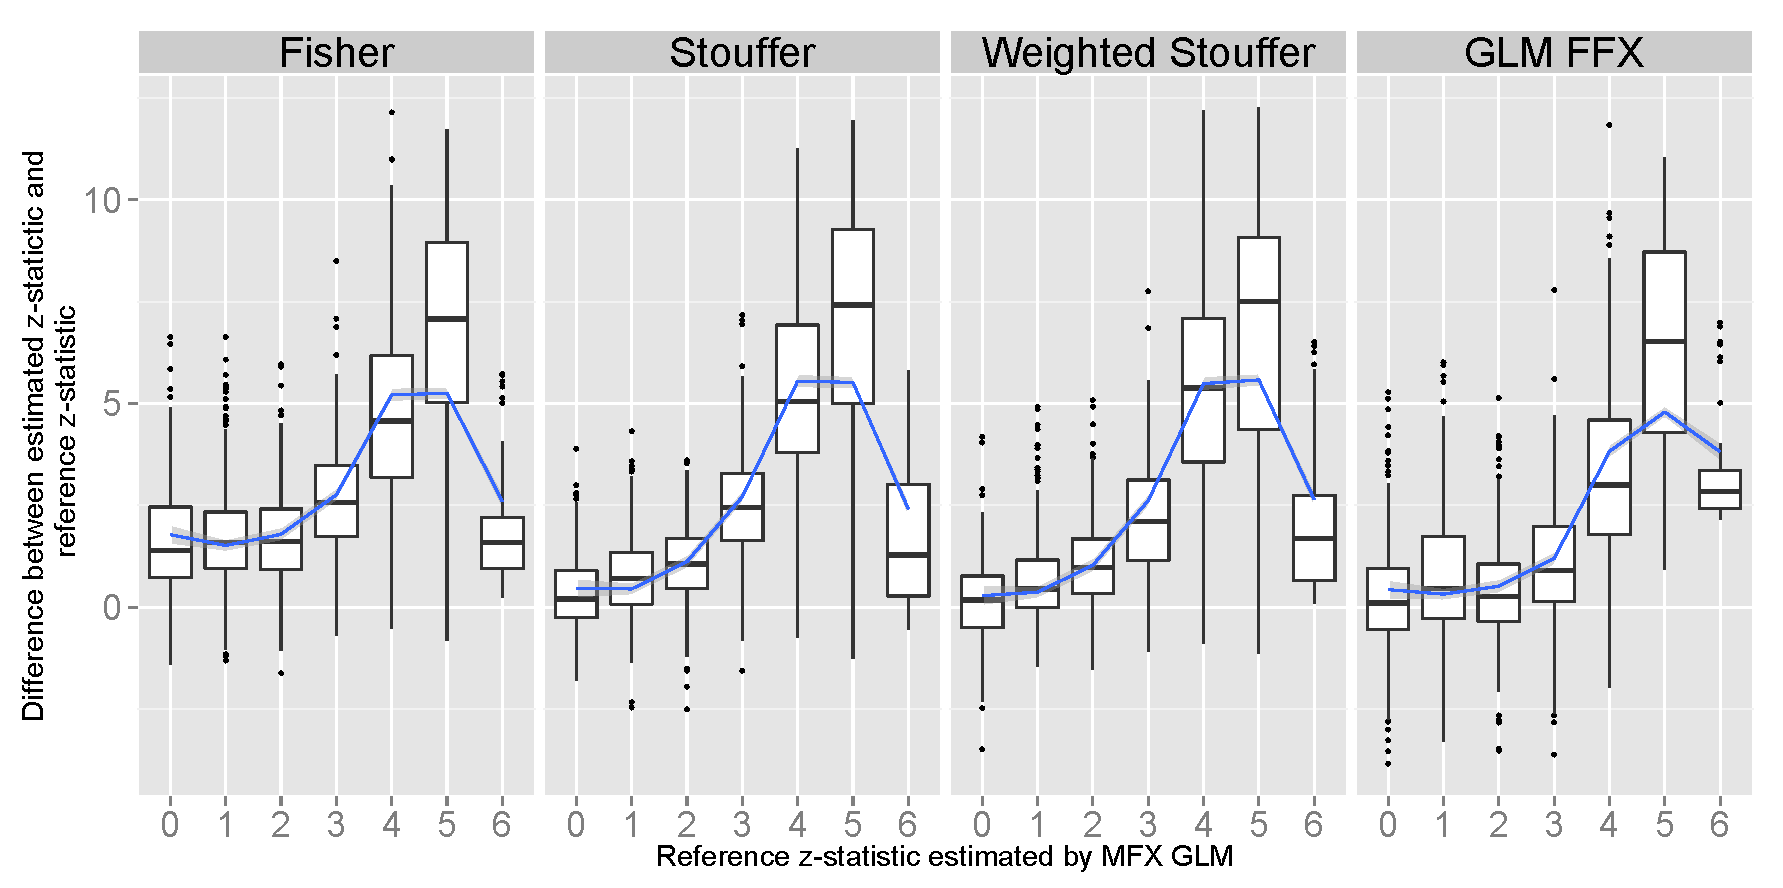
\includegraphics[width=0.8\linewidth]{./MICCAI_version/Rplot_realdata_ffx.pdf}
% 	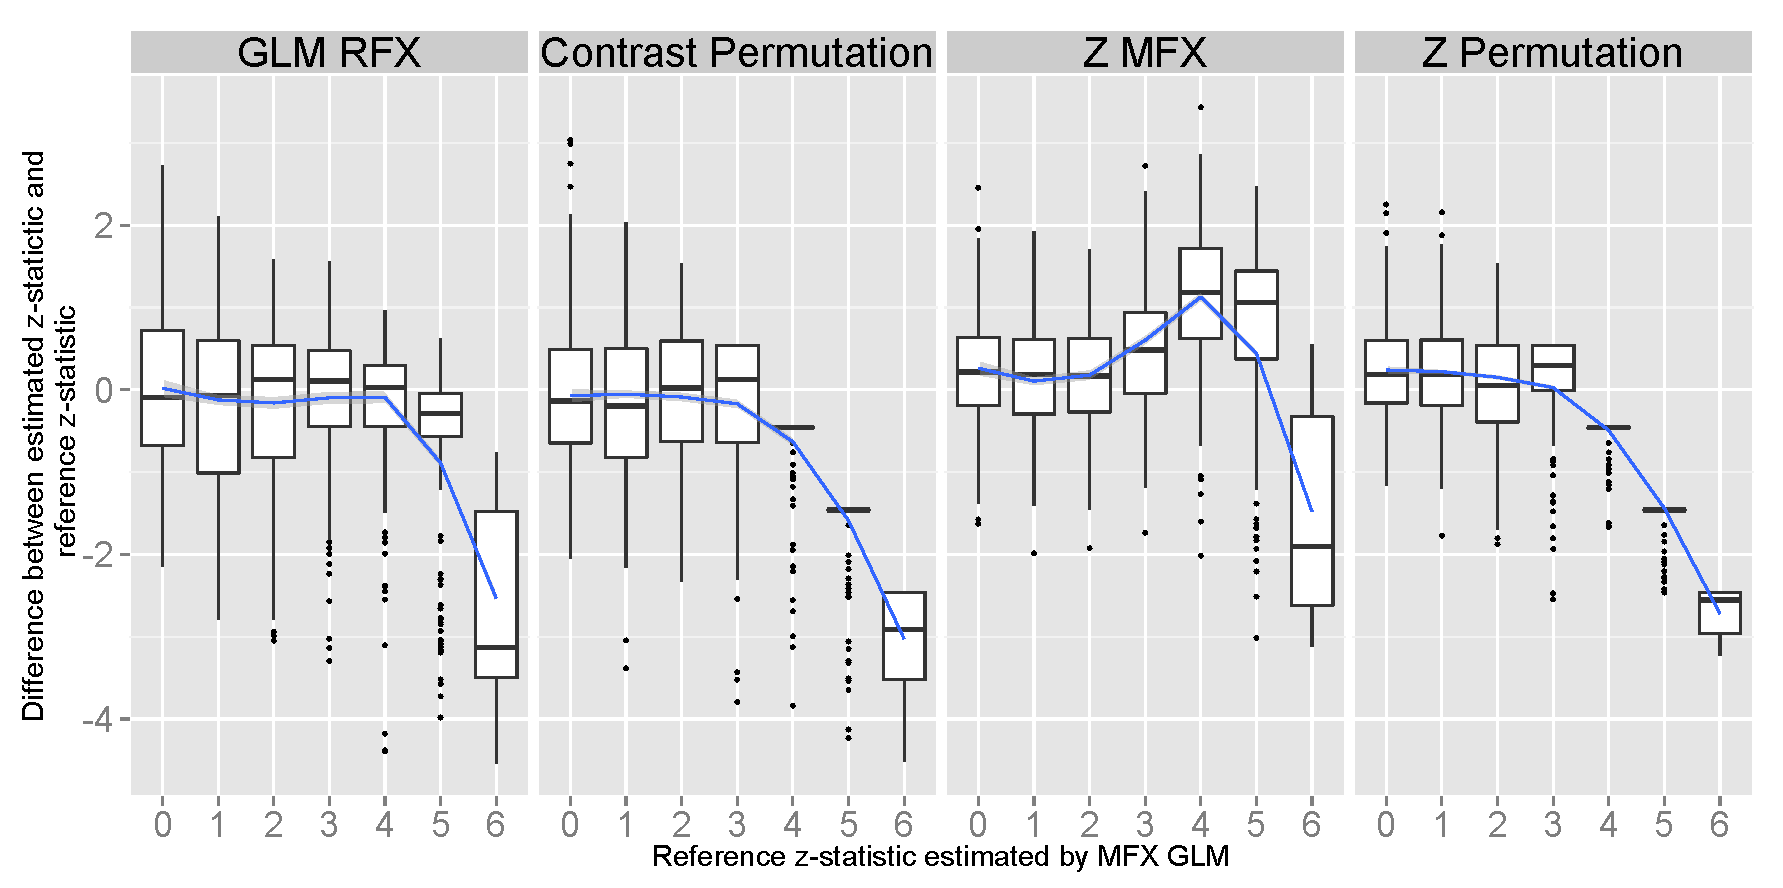
\includegraphics[width=0.8\linewidth]{./MICCAI_version/Rplot_realdata_rfx.pdf}
	\caption{Difference between the z-score estimated from each meta-analytic approach and the reference z-score from MFX GLM as a function of reference z-score.}
	\label{fig_realdata}
\end{figure}


Fig.~\ref{fig_realdata} plots the difference between the z-score estimated by each meta-analytic approach against the reference z-score computed with MFX GLM. All FFX statistics provide overly optimistic z-estimate suggesting, again, that study heterogeneity is present in the studied dataset.
Among the RFX meta-analytic approaches, GLM RFX and contrast permutations provide z-scores estimate that are equal or smaller than the reference. Z permutation provides slightly larger z-scores between 1 and 3 (reference p-values between 0.16 and 0.0013) but is mostly in agreement with the reference z-scores. On the other hand, Z MFX is more liberal than the reference for z-score ranging from 3 to 5 (reference p-values between 0.0013 and 2.9e-07) and more stringent for z-scores smaller than 5.

% Fig. 1 shows the Bland-Altman plots comparing Z-scores from the Stouffer's and weighted-Z methods each compared with the ground truth Z-scores. Overall, both approaches present the same pattern of overestimation of the Z-scores. The weighted-Z approach provides a somewhat more condensed pattern suggesting a closer match to the ground truth.
% The dice similarity score for uncorrected p-values of 0.001, 0.01 and 0.05 were 0.84, 0.87 and 0.89 respectively for Stouffer's method and 0.86, 0.88 and 0.90 for the weighted Z-score, showing again slightly better results for the weighted-Z approach. These scores are notably higher (dice similarity scores range from 0 to 1) than the scores obtained with coordinate-based meta-analyses (around 0.5, [5]).
% Finally the ROC curves displayed in figure 2 for a ground truth obtained with an FDR corrected threshold p<0.05 demonstrate again a slight advantage of weighted-Z FFX over Stouffer's FFX.

% Dice among valids
% \begin{enumerate}
% \item StouffersMFX: 0.9454
% \item PermutZ: 0.9450
% \item GLMRFX: 0.8994
% \item PermutCon: 0.8991
% \end{enumerate}

% \begin{enumerate}
% \item WeightedZ: 0.9244
% \item Stouffers: 0.9184
% \item GLMFFX: 0.8972
% \item fishers: 0.8382
% \end{enumerate}

% AUC between 0 and 0.1
% among valids
% \begin{enumerate}
% \item StouffersMFX: 0.8924
% \item PermutZ: 0.8919
% \item GLMRFX: 0.7809
% \item PermutCon: 0.7815
% \end{enumerate}

% \begin{enumerate}
% \item  WeightedZ: 0.8293
% \item  Stouffers: 0.8619
% \item  fishers: 0.6329
% \item  GLMFFX: 0.6111
% \end{enumerate}
    

\section{Conclusion}\label{sec_ccl}
We have compared eight meta-analytic approaches in the context of one-sample test. Through simulations, we found the expected invalidity of standard FFX approaches in the presence of study heterogeneity, but also of FFX GLM even with no between-study variation. In a real dataset of 21 studies of pain, there was evidence for substantial between-study variation that supports the use of RFX meta-analytic statistics. When only contrast estimates are available, RFX GLM was valid. This is in line with previous results on within-group one-sample t-tests studies~\cite{Mumford2009}. When only standardised estimates are available, permutation is the preferred option as the one providing the most faithful results. Further investigations are needed in order to assess the behaviour of these estimators in other configurations, including meta-analyses focusing on between-study differences.


\section{Acknowledgements}
We gratefully acknowledge the use of this data from the Tracey pain group, FMRIB, Oxford.

%
% ---- Bibliography ----
\bibliographystyle{plain}
\bibliography{ibma}

% %
% \begin{thebibliography}{5}
% %
% \bibitem {clar:eke}
% Clarke, F., Ekeland, I.:
% Nonlinear oscillations and
% boundary-value problems for Hamiltonian systems.
% Arch. Rat. Mech. Anal. 78, 315--333 (1982)

% \bibitem {clar:eke:2}
% Clarke, F., Ekeland, I.:
% Solutions p\'{e}riodiques, du
% p\'{e}riode donn\'{e}e, des \'{e}quations hamiltoniennes.
% Note CRAS Paris 287, 1013--1015 (1978)

% \bibitem {mich:tar}
% Michalek, R., Tarantello, G.:
% Subharmonic solutions with prescribed minimal
% period for nonautonomous Hamiltonian systems.
% J. Diff. Eq. 72, 28--55 (1988)

% \bibitem {tar}
% Tarantello, G.:
% Subharmonic solutions for Hamiltonian
% systems via a $\bbbz_{p}$ pseudoindex theory.
% Annali di Matematica Pura (to appear)

% \bibitem {rab}
% Rabinowitz, P.:
% On subharmonic solutions of a Hamiltonian system.
% Comm. Pure Appl. Math. 33, 609--633 (1980)

% \end{thebibliography}


\end{document}

%%
%% End of file `elsarticle-template-1-num.tex'.